\section{Start with a tractable research claim}
\label{sec:scope}
\subsection{The project you are actually building}
Your long-term objective is reliable reconstruction of sharp QDM magnetic images under uncertain measurement geometry. The first paper should answer a bounded version: \emph{for a single planar source layer, can joint standoff inference improve reconstruction of the magnetic field at a fixed reference plane, including on source geometries excluded from training?} FOV, sampling, and noise robustness become explicit challenge sets. Multilayer separation and optical inversion are later extensions with different identifiability assumptions.

You have access to an extensive existing COMSOL database, GPUs, real QDM measurements, and the experimental dataset underlying Bathla et al.~\cite{bathla}. Use these resources as the core of the study. The few geometries visible in the current repository do not describe the full database available to your group. This guide has not inspected that external database: counts, units, available components, calibrated heights, and acquisition labels must be established by the audit in Section~\ref{sec:data}.

\begin{tcolorbox}[title=\textbf{A one-sentence working claim}]
We investigate a joint calibration-and-reconstruction method that uses analytical propagation and a learned source prior to estimate effective standoff and reconstruct a near-plane magnetic field, with source-level holdouts and calibrated treatment of ambiguous observations.
\end{tcolorbox}

\subsection{Four hypotheses to investigate separately}
\begin{enumerate}
\item \textbf{H1: calibration matters.} Height errors explain a measurable part of reconstruction error after boundary and sampling effects are controlled.
\item \textbf{H2: joint inference helps.} Refining image and distance together improves over a height predictor followed by a fixed reconstruction network under matched training data and compute.
\item \textbf{H3: ambiguity should be represented.} A distribution or set of height--image hypotheses yields fewer confidently incorrect decisions than a single estimate.
\item \textbf{H4: physical metadata helps transfer.} Explicit observation operators and physical pixel spacing improve transfer across FOV and sampling changes.
\end{enumerate}
H1 can be rejected. H2 can be rejected. A simple baseline winning is useful information. Choose one central methodological claim for the paper; treat the other hypotheses as controls or supporting studies.

\subsection{Use the guide in passes}
\begin{tabularx}{\linewidth}{P{22mm}YY}
\toprule Pass & Read and execute & Required output before expanding scope\\\midrule
First 10 days & Scope, dataset audit, E00--E03 & Trusted operator; wrong-height curve; source split\\
Weeks 3--6 & Baselines and architecture A0--A3 & A clear baseline failure and an interpretable prototype\\
Weeks 7--12 & One proposed mechanism; challenge sets & Matched ablation with repeatable benefit\\
Months 4--6 & Real-data validation and paper evidence & Defensible physical claim, limitations, reproducible release\\\bottomrule
\end{tabularx}

\deliver{Your immediate milestone is one figure showing reconstruction error and observation mismatch versus assumed height, evaluated on several independent COMSOL source layouts.}

\section{Physics, observations, and identifiability}
\label{sec:physics}
\subsection{Define the output before defining the network}
Let $h$ be the sensor height relative to a declared source plane, and let $z_{\rm ref}$ be the fixed target-plane height. Initially use $z_{\rm ref}=0.5\um$ to match the repository. The propagation gap is $\delta=h-z_{\rm ref}>0$.
Let $x$ denote the vector field at that plane on a \emph{larger physical domain}, before restricting it to the requested output ROI. The observation is
\begin{equation}
 y=\C\Samp\mathcal Q\A_{\delta}x+\eta
   =\mathcal M_hx+\eta.\label{eq:obs}
\end{equation}
Here $\mathcal Q$ projects onto measured NV axes or selects vector components; $\Samp$ integrates/resamples to detector pixels; $\C$ restricts the observation window; and $\eta$ denotes noise. Known optical and NV-depth averaging can eventually enter $\mathcal M_h$. They should be accounted for as nuisance effects when material, even while optical \emph{deconvolution} remains outside the first paper.

For simulation inputs, $y$ can contain all three signed components. The published Bathla acquisition uses a single NV-axis projection. A model must support the actual available channels; a single-axis image cannot be relabelled as three independently measured components. The primary target is a magnetic field, not an optical photograph or binary wire segmentation.

\begin{figure}[htbp]\centering
\begin{tikzpicture}[node distance=6mm]
\node[block] (src) {Physical source\\$J$ or $\mathbf M$};
\node[block,right=of src] (ref) {Reference-plane\\field $x$};
\node[block,right=of ref] (prop) {Propagation\\$\A_{h-z_{\rm ref}}$};
\node[block,below=of prop] (sense) {Projection and\\pixel integration};
\node[block,left=of sense] (crop) {FOV restriction\\$\C$ and noise};
\node[block,left=of crop] (obs) {Observed map $y$\\and metadata};
\draw[arrow] (src)--(ref);\draw[arrow] (ref)--(prop);
\draw[arrow] (prop)--(sense);\draw[arrow] (sense)--(crop);\draw[arrow] (crop)--(obs);
\end{tikzpicture}
\caption{The observation model. Generate the physical field on a larger domain before sensing and cropping. The learned inverse estimates the target field and calibration parameters from the observed map.}
\end{figure}

\subsection{Analytical propagation and sensitivity to distance}
In a homogeneous source-free region, $\nabla\times\mathbf H=0$ and $\nabla\cdot\mathbf H=0$. The scalar potential is harmonic. For spatial frequency $\mathbf f=(f_x,f_y)$ in cycles per micrometre,
\begin{equation}
 \widehat x(\mathbf f,z_2)=e^{-2\pi\norm{\mathbf f}(z_2-z_1)}\widehat x(\mathbf f,z_1).
\end{equation}
The three signed components share this decay. In vacuum, $\mathbf B=\mu_0\mathbf H$; store which quantity and units are supplied. In this project the cache is in tesla and loading typically converts to microtesla. $B_{\rm norm}$ is nonlinear and should not be treated as another independent linear measurement channel.

\begin{equation}
 H_\delta(\mathbf f)=e^{-2\pi\norm{\mathbf f}\delta},\qquad
 \partial_h H_\delta=-2\pi\norm{\mathbf f}H_\delta.
\end{equation}
An overestimate $\Delta h$ in a direct inverse multiplies the reconstructed spectral amplitude by $e^{2\pi\norm{\mathbf f}\Delta h}$. At $f=0.5$ cycles/$\mu$m and $\Delta h=0.2\um$, this factor is about $1.87$. This is an analytical illustration, not a measured error bound for a regularized network.

\begin{figure}[htbp]\centering
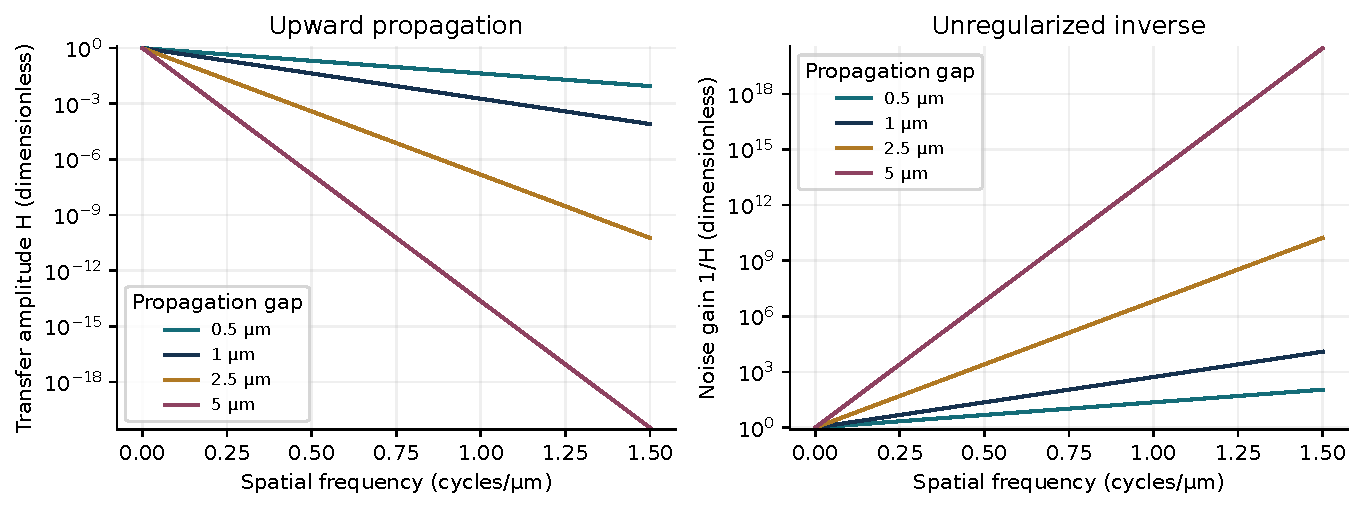
\includegraphics[width=\linewidth]{figures/propagation_and_inverse.pdf}
\caption{Original analytical illustration. Standoff attenuates fine structure and direct inversion amplifies its noise. No experimental reconstruction results are shown.}
\end{figure}
\begin{figure}[htbp]\centering
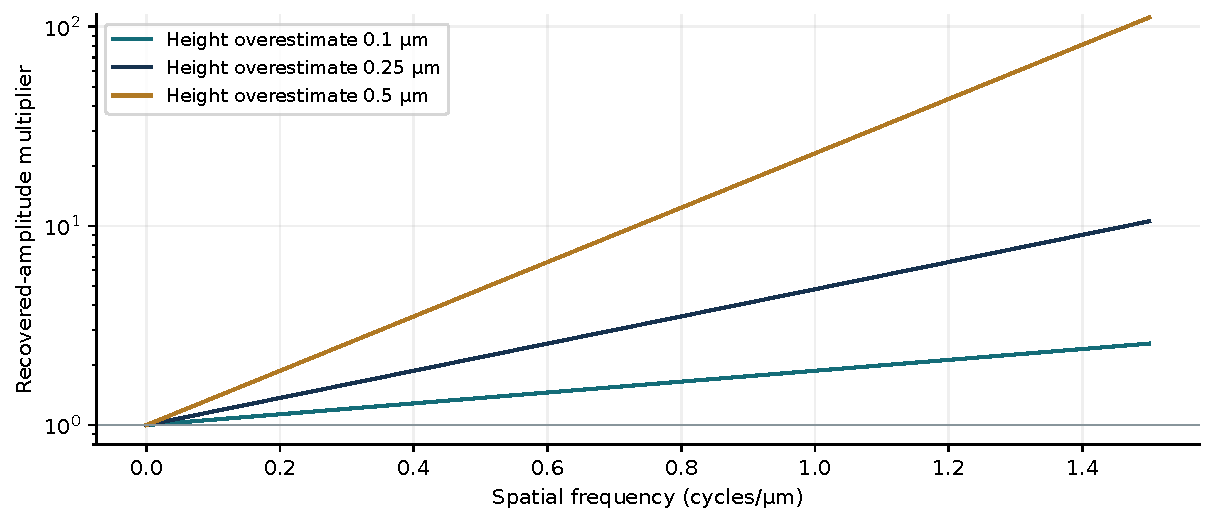
\includegraphics[width=.9\linewidth]{figures/height_sensitivity.pdf}
\caption{Original analytical illustration of distance sensitivity. A fixed height error causes greater spectral distortion at higher frequency. This motivates testing uncertainty-sensitive refinement.}
\end{figure}

\subsection{An exact reason that residual-only height estimation fails}
\begin{figure}[htbp]\centering
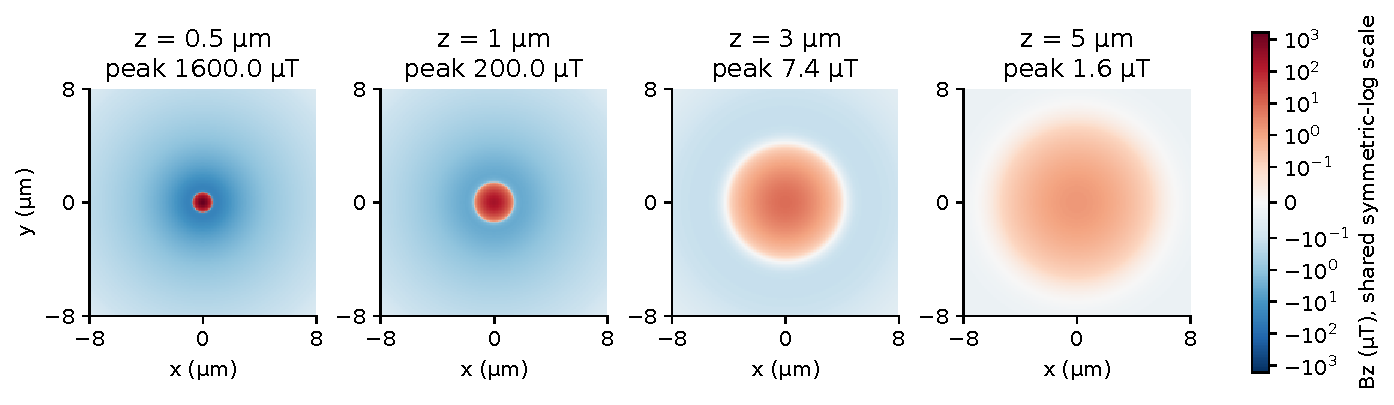
\includegraphics[width=\linewidth]{figures/dipole_height_demo.pdf}
\caption{Original analytical point-dipole example, not a COMSOL or microscope result. A common symmetric-log colour scale exposes both attenuation and broadening; peak values are stated explicitly. This example teaches observation physics, not the proposed coil benchmark.}
\end{figure}
In an ideal infinite-plane, noiseless model, suppose $y=\A_\delta x$. For any $0\leq\delta'\leq\delta$, define $x'=\A_{\delta-\delta'}x$. The semigroup property gives
\begin{equation}
 \A_{\delta'}x'=\A_{\delta'}\A_{\delta-\delta'}x=\A_\delta x=y.
\end{equation}
Thus a smoother reference field at a smaller gap explains the same observation exactly. A flexible unconstrained field can trade source structure against distance. A network trained on one coil size may learn that size as a shortcut and call larger coils ``farther away.''

Restrictions to real source families, geometric knowledge, controlled drive currents, and independent calibration can make height inference informative. A learned estimate is conditional on those assumptions. Physical consistency and extra vector channels improve practical constraints but do not guarantee unique absolute depth for unrestricted planar sources.

\subsection{Profile objectives and nuisance parameters}
A useful diagnostic is
\begin{equation}
 \Phi(h)=\min_x \left\{\tfrac12\norm{W(\mathcal M_hx-y)}^2+\lambda\R(x)\right\},
\end{equation}
where $W$ whitens the assumed noise. Plot $\Phi(h)$, its data term, and ground-truth reconstruction error separately. Profile minima depend on the prior, noise model, support, and solver accuracy; a profile is not automatically a calibrated posterior.

For local source parameters $\vartheta$, define the whitened sensitivities $J_h=\partial_h(W\mathcal M_hx_\vartheta)$ and $J_\vartheta=\partial_\vartheta(W\mathcal M_hx_\vartheta)$. A local nuisance-adjusted information diagnostic is
\begin{equation}
 \mathcal I_{h\mid\vartheta}=J_h^T(I-P_{J_\vartheta})J_h,
\end{equation}
with $P$ the projection onto the nuisance sensitivity span. If distance changes can be reproduced by changing geometry or current, little information remains. This is a local idealized diagnostic; nonlinear multimodality and model error require explicit tests.

\subsection{What additional heights actually provide}
Measurements at several heights above all sources are related by upward continuation in the ideal complete-plane source-free model. They do not independently determine an arbitrary multilayer decomposition. In practice they can improve SNR, registration checks, noise characterization, and finite-window constraints. Known stage increments give relative distances; absolute standoff remains a separate calibration question.

\subsection{A minimal physically constrained source representation}
For planar currents, a stream function $g$ can define $J_x=\partial_y g$ and $J_y=-\partial_x g$, enforcing $\nabla\cdot J=0$ away from contacts. Predicting $g$ and using Biot--Savart provides a source-aware prior, then the field at $z_{\rm ref}$ becomes the main output. Contacts and currents crossing the FOV require appropriate source-domain extensions and boundary treatment. Field-first and source-latent formulations should be compared, not silently conflated.

\caution{Standoff deblurring restores detail conditional on a prior and measurement model. A finer output grid is not evidence of finer physical resolution. Define success through recoverable features, field accuracy, calibration accuracy, and reliability on held-out sources.}
